\cotefile{134-2}
\scanpage{95}
\mspage{\unsure{\ldots)|2}}
had been done and the homotopy category expressed in terms of $\infty$-groupoids. But finally it appears this is not so, they have been working throughout with a notion of $\infty$-groupoid too restrictive for the purposes I had in mind (probably because they insist I guess on strict associativity of compositions, rather than associativity up to a (given) isomorphism\inserted{\handwritten{or rather, homotopy}}) - to the effect that the simply connected homotopy types they obtain are merely products of Eilenberg-MacLane spaces, too bad ! They do not seem to have realized yet that this makes their set-up wholly unadequate \handwritten{\unsure{as}} a sweeping foundational set up for homotopy. This brings to the fore again to work out the suitable definitions for $n$-groupoids - if this is not done yet anywhere. I spent the afternoon today trying to figure out a reasonable definition, to get a feeling at least of where the difficulties are, if any. I am guided mainly of course by the topological interpretation. It will be short enough to say how far I got. The main part of the structure it seems is expressed by the sets $F_i$ ($i\in\underline{N}$) of $i$-objects, the source, target and identity maps
\[
\begin{aligned}
s^i_1,t^i_1 &: F_i\longrightarrow F_{i-1} &&(i\geq 1)\\
k^i_1 &: F_i\longrightarrow F_{i+1} &&(i\in\underline{N})
\end{aligned}
\]
\margin{\handwritten{\uline{NB} we write also $\mathrm{id}_a$ instead of ${\unsure{K|k}}^i_1(a)$ and $\check{u}$ for $\mathrm{inv}_i(u)$}}
and the symmetry map (passage to the inverse)
\[
\mathrm{inv}_i:\quad F_i\longrightarrow F_i\qquad(i\geq 1)
\]
satisfying some obvious relations : $k^i_1$ is right inverse to the \deleted{target} source and target maps $s_1^{i\deleted{\unsure{-}}+1}$, $t_1^{i+1}$, $\mathrm{inv}_i$ is an involution and ``exchanges'' source and target, and moreover for $i\geq 2$
\[
\begin{aligned}
s^{i-1}_1s^i_1&=s^{\deleted{\unsure{i-1}}i-1}_1t^i_1 &&(\mathrel{\overset{\mathrm{def}}{=}}s^i_2:F_i\longrightarrow F_{i-2})\\
t^{i-1}_1s^i_1&=t^{i-1}_1t^i_1 &&(\mathrel{\overset{\mathrm{def}}{=}}t^i_2:F_i\longrightarrow F_{i-2})\quad;
\end{aligned}
\]
\unsure{thus|thur} the composition of the source and target maps yields, for $0\leq j\leq i$, just \uline{two} maps
\[
s^i_\ell,\ t^i_\ell:\ F_i\longrightarrow F_{i-\ell}\handwritten{=F_j}\quad(\ell=i-j)\,.
\]
The next basic structure is the composition structure, where the usual composition of arrows, more specifically of $i$-objects $(i\geq1)$ $v\circ u$ (defined when $t_1(u)=s_1(v)$) must be supplemented by the Godement-type operations $\handwritten{\mu}*\handwritten{\lambda}$ when $\handwritten{\mu}$ and $\handwritten{\lambda}$ are ``arrows between arrows'' \inserted{etc} . Following this line of thought, one \unsure{getc|gets} the composition maps
\[
(u,v)\longmapsto v\overset{\unsure{i|t}}{*}_\ell u\quad:\quad (F_i,\deleted{s}t^i_\ell)\mathbin{\mathrm{x}}_{F_{i-\ell}}(F_i,s^i_\ell)\longrightarrow F_i\ ,
\]
the $\deleted{\unsure{*_\ell}}$ \deleted{\unsure{application|operation}}\inserted{composition of} $i$-objects \inserted{$u,v$} $(1\leq\ell\leq i)$ being defined when the $\ell$-target of $u$ is equal to the $\ell$-source of $v$, and then we have
\[
\left.\begin{aligned}
\deleted{\unsure{*_\ell}}\ s^i_1(v*_\ell u)&=s^i_1(v)\underset{\unsure{1}}{*_{\ell-1}}s^i_1(u)\\
\handwritten{t^i_1(v*_\ell u)}&\handwritten{{}=t^i_1(v)*_{\ell-1}t^i_1(u)}
\end{aligned}\right\}\handwritten{\quad\ell\geq2\quad\text{i.e.}\quad\ell-1\geq1}
\]
% archive sheet number: 94
\scanpage{96}
\mspage{\handwritten{$2'$}}
and for $\ell=1$
\[
\begin{aligned}
s_1(v*_1u)&=s_1(u)\\
t_1(v*_1u)&=t_1(v)
\end{aligned}
\]
(NB the operation $v*_1u$ is the usual composition $v\circ u$).

One may be tempted to think that the preceding data exhaust the structure of $\infty$-groupoid, and that they will have to be supplemented only by a handful of suitable \uline{axioms}, one being \uline{associativity} for the operation $\overset{i}{*}_\ell$, which can be expressed essentially by saying that this composition operation turns $F_i$ into the set of arrows of a category having $F_{i-\ell}$ as set of objects (with\deleted{\unsure{s}} the source and target maps $s^i_\ell$ and $t^i_\ell$, and with identity map $k_\ell^{i-\ell}:F_{i-\ell}\longrightarrow F_i$, the composition of the identity maps $F_{i-\ell}\longrightarrow F_{i-\ell+1}\longrightarrow\ldots F_{i-1}\longrightarrow F_i$), and another being the Godement relation
\[
(v' *_{\handwritten{\alpha}}v)*_{\handwritten{\nu}}(u'*_{\handwritten{\alpha}}u)
=(v'*_{\handwritten{\nu}}u')*_{\handwritten{\alpha}}(v*_{\handwritten{\nu}}u)
\]
(with the assumptions \handwritten{$1\leq\alpha<\nu$,} \deleted{\unsure{and}} \handwritten{$u,u',v,v'\in F_i$ and}
\[
\handwritten{\left\{\begin{aligned}t_\alpha(u)&=s_\alpha(u')\\t_\alpha(v)&=s_\alpha(v')\end{aligned}\right. \qquad
t_\nu(u)=s_\nu(v)=s_\nu(v')=t_\nu(u')}
\]
\deleted{\unsure{imply}}\handwritten{\unsure{express}}ing that both members are defined), plus the two relations concerning the inversion of $i$-objects $(i\geq1)$ $u\mapsto\check{u}$,
\[
\begin{aligned}
u*_1\check{u}&=\deleted{\unsure{k_1}}\ \mathrm{id}_{t_1(u)}\ ,\qquad \check{u}*_1u=\mathrm{id}_{s_1(u)}\\
{(v*_\ell u)}^{\scriptscriptstyle\vee}&=\check{\unsure{v|u}}*_\ell\check{u}\qquad(\ell\geq2)\quad.
\end{aligned}
\]
It just occurs to me, by the way, that the \inserted{previous} description of basic (or ``primary'') data for an $\infty$-groupoid is already uncomplete in some rather obvious respect, namely that the symmetry-operation \inserted{\handwritten{$\mathrm{inv}_i:$}} $u\mapsto\check{u}$ on $F_i$ must be complemented by $i-1$ similar involutions on $F_i$, which corresponds algebraically to the intuition that when we have an \inserted{\handwritten{$(i+1)$-}}arrow $\handwritten{\lambda}$ say between two \inserted{\handwritten{$i$-}}arrows $u$ and $v$, then we must be able to deduce from it another arrow from $\check{u}$ to $\check{v}$ (namely $u\mapsto\check{u}$ has a ``functorial \unsure{caracter|character}'' \deleted{\unsure{in u}} for variable $u$)\unsure{?|;|.} This seems a rather anodine modification of the previous set-up, and is irrelevant for the main point I want to make here, namely: that for the notion of $\infty$-groupoids we are after, all the equalities just envisioned in this paragraph (and those I guess which will ensue\deleted{s} naturally by the necessary extension of the basic involution on $F_i$) should be replaced by ``homotopies'' namely by $(i+1)$-arrows between the\deleted{\unsure{r}} two members. These arrows should be viewed, I believe, as being part of the data, \deleted{the} \deleted{The diffi} they appear here as a kind of ``secondary'' structure. The difficulty which appears now is to work out the natural coherence properties
% archive sheet number: 95
\scanpage{97}
\mspage{\unsure{\ldots)|3}}
concerning this secondary structure. The first thing I could think of is the ``pentagon axiom'' for the associativity data, which occurs when looking at associativities for the compositum (for $\overset{\deleted{\unsure{i}}i}{*}_\ell$ say) of four factors. Here again\deleted{\unsure{,}} the first reflex would be to write down, as usual, an \uline{equality} for \deleted{the} two compositions of associativity isomorphisms, exhibited in the pentagon diagram. One suspects however that such equality should, again, be replaced by a ``homotopy''-arrow, which now appears as a kind of ``ternary'' structure - before even having exhausted the list of coherence \handwritten{``}relations\handwritten{''} one could think of with respect to the secondary structure ! Here one seems caught at first sight in an infinite chain of \deleted{increasingly}\inserted{\handwritten{ever}} \handwritten{``}higher\handwritten{''}, and presumably\handwritten{,} messier structures, where one is going to get hopelessly lost, unless one discovers some simple guiding principle for sheding some clarity in the mess.

\handwritten{3.}\quad I thought of writing you mainly because I believe that, if anybody, you should know if the kind of structure I am looking for has been worked out - maybe even \uline{you} did ? In this respect, I vaguely remember that you had a description of $n$-categories in terms of $n$-semisimplicial sets, satisfying certain exactness conditions, in much the same way as an ordinary category can be interpreted, via its ``nerve'', as a particular type of semisimplicial set. But I have no idea if your definition applied only for describing $n$-categories with strict associativities, or not.

Still some comments in the spirit of your axiomatics of homotopical algebra - in order to make the question I am proposing more seducing maybe to you ! One comment is that presumably, the category of $\infty$-groupoids (which is still to be defined) is a ``model category'' for the usual homotopy category; this would be at any rate one plausible way to make explicit the intuition referred to before, that a homotopy type is ``essentially the same'' as an $\infty$-groupoid up to $\infty$-equivalence. The other comment: the construction of the fundamental $\infty$-groupoid of a space, disregarding for the time being the question of working out in full the pertinent structure on this messy object, can be paraphrased in any model category in your sense, and yields a functor from this category to the category of $\infty$-groupoids, and hence (by geometric realization, or by \unsure{localisation|localization}) also to the usual homotopy category. Was this functor obvious beforehand ? It is of a non-trivial nature only when the model category is \uline{not} pointed - as a matter of fact the whole construction can be carried out canonically, in terms of a ``cylinder object'' $\unsure{I|\mathbb{I}}$ for the final object $e$ of the model category\handwritten{, playing the role of the unit segment.}
% archive sheet number: 96
\scanpage{98}
\mspage{\handwritten{$4'$}}
Its high time to stop this letter - please excuse me if it should come ten or fifteen years too late, or maybe one year t\deleted{\unsure{t}}oo early. If you are not interested for the time being in such general nonsense, maybe you know someone who is \ldots

Very cordially yours\\
\handwritten{Alexander}\\
% archive sheet number: 97
\scanpage{99}
\mspage{\handwritten{4}}
\hfill\unsure{20.2.}\\
I finally went on pondering about a definition of $\infty$-groupoids, and \handwritten{it} seems to me that, after all, the topological motivation does furnish the ``simple guiding principle'' which yesterday seemed to me to be still to be discovered, \inserted{\handwritten{in order}} not to get lost in the \unsure{messyness|messiness} of ever higher order structures. Let me try to put it down roughly.

\handwritten{4.}\quad First I would like to correct somewhat the rather undiscriminate description I gave yesterday of what I thought of viewing as ``primary'', secondary, ternary etc structures for an $\infty$-groupoid. More careful refletion conduces to view as the most primitive, starting structure on the set of sets $F_i$ ($i\in\underline{N}$), as a skeleton on which progressively organs and flesh will be added, the mere data of the source and target maps
\[
s_i,t_i:F_i\rightrightarrows F_{i-1}\qquad(i\geq1)\ ,
\]
which it will be convenient to supplement \deleted{by the} formally by corresponding maps $s_0,t_0$ for $i=1$, from $F_0$ to $F_{-1}\mathrel{\overset{\mathrm{def}}{=}}$ one-element set. In a moment we will pass to a universal situation, when the $F_i$ are replaced by the corresponding ``universal'' objects $\underline{F}_i$ in a suitable catégory stable under finite products, where $F_{-1}$ will be the final element. For several reasons, it is not proper to view the inversion maps $\mathrm{inv}_i:F_i\to F_i$, and still less the other $i-1$ involutions on $F_i$ which I at first overlooked\handwritten{,} as being part of the primitive or ``skeletal'' structure. One main reason is that already for the most usual $2$-groupoids, such as the $2$-groupoid whose $0$-objects are ordinary ($1$-) groupoids, the $1$-objects being equivalences between these (namely functors which are fully faithful and essentially \unsure{surjectve|surjective}), and the $2$-objects morphisms (or ``natural transformations'') between such, there is \uline{not}, for an $1$-object $f:C\to C'$, a natural choice of an ``inverse'' namely of a quasi-inverse in the usual sense. And even assuming that such quasi-inverse is chosen for every $f$, it is by no means clear that such choice can be made involutive, namely such that $(f^{\vee})^{\vee}=f$ for every $f$ (and not merely $(f^{\vee})^{\vee}$ isomorphic to $f$). The maps $\mathrm{inv}_i$ will appear rather, quite naturally, as ``primary structure'', and they will not be involutions, but ``pseudo-involutions'' (namely involution ``up to homotopy''). It turns out that among the various functors \inserted{\handwritten{$\Pi_\infty$}} we will construct\handwritten{,} from the category of topological spaces to the category of $\infty$-groupoids\deleted{\unsure{,}} \handwritten{(}the construction depending on arbitrary choices and \unsure{yielding|yilding} a large bunch of mutually non isomorphic functors, which however are ``equivalent'' in a sense which will have to be made precise\unsure{\ldots}\deleted{-}\handwritten{)} there are choices neater than others, and some of these will yield in the primary structure maps $\mathrm{inv}_i$ which are actual involutions, and similarly for the other pseudo-involutions, appearing \deleted{\unsure{as}}\inserted{in succession as} higher order structure. The possibility of such neat and fairly natural choices had somewhat mislead me
% archive sheet number: 98
\scanpage{100}
\mspage{\handwritten{$4'$}}
yesterday.

What may look less conviencing though at first sight, is my choice to view \inserted{\handwritten{as non-primitive}} even the ``degeneration maps'' $k_1^i:F_i\to F_{i+1}$, associating to every $i$-object the $(i+1)$-object acting as an identity on the former, In all cases I have met so far, these maps are either given beforehand with the structure (of a $1$-category or $2$-category say), or they can be uniquely deduced from the axioms. In the present set-up however, they seem to me to appear more naturally as ``primary'' (not as primitive) structure, much in the same way as the $\mathrm{inv}_i$. Different choices for associating an $\infty$-groupoid to a topological space, while yielding the same base-sets $F_i$, will however (according to this point of view) give rise to different maps $k_1^i$. The main motivation for this point of view comes from the fact that the mechanism for a uniform construction of the chain of ever higher order structures makes a basic use of the source and target maps only and of their ``transposés'' (see below), and (it seems to me) \unsure{not|act} at all of the degeneration maps, which in this respect rather \handwritten{are} confusing \deleted{a}\inserted{the real} picture\handwritten{,} \inserted{\handwritten{if viewed as ``primitive''.}} - The degeneration maps rather appear as typical cases of primary structure, probably of especial significance in the practical handling of $\infty$-groupoids, but not at all in the conceptual machinery leading up to the con\deleted{\unsure{stru}}struction of the structure species \deleted{of} \handwritten{``}$\infty$-groupoids.\handwritten{''}

- Much in the same way, the composition operations $\overset{i}{*}_1$ are viewed as primary, \deleted{not} as primitive or skeletal structure. Their description for the fundamental $\infty$-groupoid of a space - for instance the description of composition of paths - depends on arbitray choices, such as the choice of an isomorphism (say) between $(I,1)\handwritten{\amalg}_e(I,0)$ and $I$, where $I$ is the unit interval, much in the same way as the notion of an inverse of a path depends on the choice of an isomorphism of $I$ with itself, exchanging the two end-points $0$ and $1$. The operations $\overset{i}{*}_2$ of Godement take sense only once the composition operations $*_1$ are defined - they are ``secondary structure'', and successively the operations $*_3\ldots *_i$ appear as ternary etc structure. This is correctly suggested by the notations which I chose\deleted{\unsure{n}} yesterday, where however \handwritten{I} hastily threw\deleted{\unsure{gh|ht}} all those operations into a same pot baptized ``primary structure''!

It is about time though to come to a tentative precise definition o\unsure{r|f} description of the process of stepwise introduction of an increasing chain of higher order structure. This will be done by introducing a canonical sequence of categories and functors
\[
\underline{C}_0\to\underline{C}_1\to\underline{C}_2\to\ldots\to\underline{C}_n\to\underline{C}_{n+1}\to\unsure{\ldots|-}\ ,
\]
% archive sheet number: 99
where $\underline{C}_n$ denotes the \deleted{``universal''} category harbouring the ``universal'' parti%
\scanpage{101}%
\mspage{\handwritten{5}}%
al structure of a\deleted{\unsure{n}} would-be $\infty$-groupoid, endowed only with its ``structure\handwritten{ of} order $\leq n$\handwritten{»}. The idea is to give a\deleted{\unsure{n}} direct inductive construction of this sequence, by describing $C_0$, and the passage from $C_n$ to $C_{n+1}$ ($n\geq0$), namely from $n$-ary to $(n+1)$-ary structure. As for the meaning of ``universal structure'', \deleted{\unsure{it depends}} once a given structure species is at hand, it depends on the type of categories (described by the exactness properties one is assuming for these) one wants to take as carriers for the considered structure, and the type of exactness properties one assumes for the functor one allows between these. The choice depends partly on the particular species;\deleted{\unsure{at|it}} if it is an algebraic structure which can be described say by a handful of composition laws between a bunch of base sets (or base-objects, when looking at ``realizations'' of the structure not only in the category (Sets)), one natural choice is to take categories with finite products, and functors which commute to these. For more sophisticated algebraic structures (including structure of category, groupoid or the like), which requires for the description of data or axioms not only finite products, but also some fiber products, one other familiar choice is to take categories with finite inverse limits, and left exact functors. \handwritten{Still} more sophisticated \deleted{choices}\inserted{\handwritten{structures}}, when the description of the structure in terms of base objects requires not only some kinds of inverse limits, but also more or less arbitrary direct limits (such as the structure of a comodule over an algebra, which requires consideration of tensor products over a ring object),%
% slanted
\margin{\handwritten{or the structure \unsure{of} \unsure{-|a} torsor under \unsure{a} group}} still \deleted{\unsure{more|much}} more stringent conditions will have to be imposed upon categories and functors between these, for the structure to make a sense in \deleted{any of} these categories, and the functors to transform a structure of this type in one category into one of same type in another. In most examples I have looked up, everything is \unsure{OK} taking categories which are topoi, and functors between these which are inverse image functors for morphisms of topoi, namely which are left exact and commute with arbitrary direct limits. Th\deleted{\unsure{er|re}}ere is a general theorem for the existence of universal structures, covering all these cases - for instance there is a ``classifying topos'' for most algebr-geometric structures, whose cohomology say should be viewed as the ``classifying cohomology'' of the structure species considered. In the case we are interested in here, it is convenient however to work with the smallest categories $C_n$ feasable - which amounts to being as generous as possible for the categories \deleted{and functors} one is allowing as carriers for the structure of an $\infty$-groupoid, and for the functors between these which are expected to carry an $\infty$-groupoid into an $\infty$-groupoid. What we will do is define ultimately a structure of an $\infty$-groupoid in a category $C$, as a sequence of objects $F_i$ ($i\in\underline{N}$), endowed with some structure to be defined,
% archive sheet number: 100
\scanpage{102}
\mspage{\handwritten{$5'$}}
% archive sheet number: 101
assuming merely that in $C$ \deleted{certain \unsure{fiber|finer}} finite products of the $F_i$ exist, plus certain \deleted{fiber products}\inserted{\handwritten{finite inverse limits}} built up with the $F_i$'s and the maps $s^i_\ell$, $t^i_\ell$ between them (the iterated source and target maps). It should be noted that the type of \deleted{fiber products}\inserted{\handwritten{$\varprojlim$}} we allow, which will have to be made precise below, is fixed beforehand in terms of the ``skeletal'' or ``primitive'' structure alone, embodied by the family of couples $(s_i,t_i)_{i\in\underline{N}}$. This implies that the \deleted{\unsure{functors}} categories $\underline{C}_i$ can be viewed as having \uline{the same set o\handwritten{f} objects}, namely the objects $\underline{F}_i$ (underlined now to indicate their universal nature, and including as was said before $\underline{F}_{-1}=$ final object), plus the finite products and \inserted{\handwritten{iterated}} fiber products of \deleted{the type} so-called ``standar\deleted{\unsure{d}}\handwritten{t}'' type. While I am writing, it appears to me \deleted{\unsure{now|that}} even that the finite products \inserted{\handwritten{here}} are of no use (so we just drop them both in the condition on categories which are accepted for harbouring $\infty$-groupoids, and in the set of objects of the categories $C_i$). Finally, the common set of objects of the categories $\underline{C}_i$ is the set of ``standart'' \inserted{\handwritten{iterated}} fiber products of the $\underline{F}_i$, built up using only the primitive structure embodied by the maps $s_i$ and $t_i$ (which I renounce to underline !). This at the same time gives, in principle, a\deleted{\unsure{n}} precise definition of $\underline{C}_0$, at least up to equivalence - it should not be hard anyhow to give a wholly explicit description of $\underline{C}_0$ as a small category, having a countable set of objects, ,once the basic notion of the standart \inserted{\handwritten{iterated}} fiber-products has been explained.

Once $\underline{C}_0$ is constructed, we will get the higher order categories $\underline{C}_1$ (primary), $\underline{C}_2$ etc by an \uline{inductive process of succesively adding arrows} The category $\underline{C}_\infty$ will then be defined as the direct limit of the categories $\underline{C}_n$, having same objects t\handwritten{he}refore as $\underline{C}_0$, with
\[
\mathrm{Hom}_\infty(X,Y)=\varinjlim_n\mathrm{Hom}_n(X,Y)
\]
for any two objects. This being done, giving a structure of $\infty$-groupoid in any\deleted{ allowable} category $C$, will amount to giving a functor
\[
\underline{C}_\infty\longrightarrow C
\]
commuting with the standar\handwritten{t} \inserted{\handwritten{iterated}} fiber products. This can be reexpressed\handwritten{,} as amounting to the same as to give a sequence of objects $(F_i)$ in $C$, \deleted{such} and maps $s^i_1,t^i_1$ between these, satisfying the two relations I \unsure{wrote|write} down yesterday (page $2$) (and which of course have to be taken into account when defin\deleted{\unsure{f}}ing $C_0$ \deleted{\unsure{s}}to start with, I forgot to say\deleted{\unsure{t}} before), and such tha\unsure{t} standart fiber products defined in terms of these data should exist in $\unsure{F|C}$,%
% slanted
\margin{\handwritten{I'll drop the \unsure{qualification} ``iterated'' henceforth!}} plus a bunch of maps \deleted{from}\inserted{between} these fiber-products \deleted{\unsure{to}} (in fact, it will suffice to give such maps with target among the $F_i$'s), satisfying certain relations embodied in the structure of the category $\underline{C}_\infty$. I am convinced that this bunch of maps (namely the maps stemming from arrows in $\underline{C}_\infty$) not only is infinite, but cannot either be generated in the
\scanpage{103}
\mspage{\handwritten{6}}
obvious sense by a finite number, nor even by a finite number of infinit\unsure{e} series of maps such as $k_{\deleted{\unsure{1}}\handwritten{\ell}}^i$, $\mathrm{inv}_i$, $\overset{i\deleted{\unsure{\ell}}}{*}_\ell$, the compatibility arrows in the pentagon, and the like. More precisely still, I am convinced that none of the functors $\underline{C}_n\to\underline{C}_{n+1}$ is an equivalence, which amounts to saying that the structures of increasing order form a\deleted{\unsure{n}} strictly increasing sequence - at every step, there is actual extra structure added.%
% slanted
\margin{\handwritten{\uline{\unsure{NB}} That $\overset{i}{*}_\ell$ is \unsure{of} order $\ell$ and not $\unsure{i|\ell-1}$ is heuristically \unsure{clear}, but will \unsure{need} a proof none the less!}}
 This is perhaps evident beforehand to topologists in the know, but I confess that for the time being it isn't to me, in terms uniquely of the somewhat formal description I will make of the passage of $\underline{C}_n$ to $\underline{C}_{n+1}$. \deleted{which}\inserted{\handwritten{This step}} theoretically is all that remains to be done, in order to achieve an explicit construction of the \deleted{notion of an} structure species of an \deleted{\unsure{$\infty$}}$\infty$-category (besides the definition of standart fiber products) - without having to get involved still less lost in the technical intricacies of ever messier diagrams to\deleted{\unsure{,}} write down, with increasing order of the structure\deleted{\unsure{s}} to be added \ldots

\handwritten{6.}\quad In the outline of a method of construction for the structure species, there has not been any explicit mention so far \unsure{of|af} the topological motivation behind the whole approach, which could wrongly give the impression of being a purely algebraic one. However, topological considerations alone are giving me the clue both for the description of the so-called standart fiber products, and of the inductive step allowing to wind up from $\underline{C}_n$ to $\underline{C}_{n+1}$ \unsure{?|.} The heuristics \deleted{\unsure{th}}\handwritten{indeed} of the present approach is simple enough, and suggested by the starting task, to define pertinent structure on the \inserted{system of} sets $F_i(X)$ of ``homotopies'' of arbitrary order, associated to an arbitrary topological space. In effect, the functors \deleted{\unsure{$X\longrightarrow F$}}
\[
X\longmapsto F_i(X)
\]
are representable by spaces $D_i$, which are easily seen to be $i$-cells. The source and target maps $s^i_1,t^i_1:F_i(X)\rightrightarrows F_{i-1}(X)$ are transposed to maps, which I may denote by the same \deleted{\unsure{set}}\handwritten{lett}ers
\[
s^i_1,t^i_1:\quad D_{i-1}\rightrightarrows D_i\,.
\]
Handling around a little, one easily convinces oneself that all the main structural items on $F_*(X)$ which one is figuring out in succession, such as the degeneracy maps $k_1^i$, the inversion maps $\mathrm{inv}_i$, the composition $v\bullet u=v*_1u$ for $i$-objects, etc, are all transposed of similar maps which are defined between the cells\deleted{\unsure{s}} $D_i$, or which go from such cells to certain spaces, deduced from these by gluing them together - the most evident example \inserted{in this respect} being the composition of paths, which is transposed of a map from the unit segment $\inserted{I=}D_1$ into $(I,1)\amalg_e(I,0)$, having preassigned values on the \unsure{endpoints|andpoints} of $I$ \handwritten{(}which correspond in fact to the images of the two maps $s_1^1$, $\unsure{t_1 1|t_1^1}:D_0={}\text{one point}\rightrightarrows D_1=I$\handwritten{)}.
% archive sheet number: 102
\scanpage{104}
\mspage{\handwritten{$6'$}}

In a more suggestive way, we could say \deleted{\unsure{that}}\unsure{from|thus} this experimenting that the family of discs $(D_i)_{i\in\underline{N}}$, together with the maps $s,t$ and a lot of extra structure which enters into the picture step by step, is what we would like to call a \uline{co}-$\infty$-\uline{groupoid in the category} (Top) of \unsure{topologica|topological} spaces (namely an $\infty$-groupoid in the dual category $(\mathrm{Top})^o$), and that the structure of $\infty$-category on $F_*(X)$ we want to describe is the transform of this co-structure into an $\infty$-groupoid, by the contravariant functor from (\unsure{Tp|Top}) to (Sets) defined by $X$. The \inserted{\handwritten{(iterated)}} amalgamated sums in (Top) which allow to glue together \deleted{\unsure{the|these}} various $D_i$'s using the $s$ and $t$ maps between them, namely the corresponding fibered products in $(\mathrm{Top})^o$, are indeed transformed by the functor $h_X$ into fibered products of (Sets).
The suggestion is, moreover, that if we view our co-structure in (Top) as a co-structure in the subcategory of Top, say $B_\infty$, whose objects are the \deleted{\unsure{$D_i$}}cells $D_i$ and the amalgamated sums \deleted{\unsure{r|s}}built up with these which step-wise enter into play, and whose arrows are all those arrows which are introduced stepwise to define the co-structure, and all compositions of these - that \deleted{\unsure{it}}\handwritten{this} \deleted{\unsure{t}}should be \deleted{\illegible{1}}\uline{\handwritten{the} universal structure} in the sense dual to the one we have been contemplating before; or what amounts to \deleted{th} the same, that the corresponding $\infty$-groupoid structure in the dual category $B_\infty^o$ is ``universal'' - which means essentially that it is none other than the universal structure in the category $\underline{C}_\infty$ we are after.

Whether or not this expectation \deleted{\unsure{be|is}}\inserted{\handwritten{will turn out to be}} correct (I believe it is\handwritten{$^{*}$}), we should
% slanted
\margin{\handwritten{* (23.2) But no longer now - and \unsure{I} do not really care!}}
be aware that, while the successive introduction of maps between the cells $D_i$ and their ``standart'' amalgamated sums (which we will define precisely below) depends at every stage on arbitrary choices, the catego\deleted{ry}ries $\underline{C}_n$ and their limit $\underline{C}_\infty$ do not depend on any \inserted{of these} choices ; assuming the expectation is correct, this means that up to (unique) isomorphism, the category $B_\infty$ (and each of the category $B_n$ of which it appears as the direct limit) is independant of those choices - the isomorphism between two such categories transforming any one choice made for the first, into the corresponding choice made for the second. Also, while this expectation was of course the crucial motivation leading to the explicit description of $\underline{C}_0$ and of the \inserted{inductive} step from $\underline{C}_n$ to $\underline{C}_{n+1}$, this description seems to me a reasonable one and in any case it makes a formal sense, \inserted{\handwritten{quite}} independently of whether the expectation proves valid or not

\handwritten{7.} Before pursuing, it is time to give a more complete discription of the primitive structure on $(D_i)$, as embodied by the maps $s,t$, which I will now denote by
\[
{\unsure{\phi|\delta|\varnothing}}_i^+,\,\phi_i^-:D_i\rightrightarrows D_{i+1}.
\]
It appears that these maps are injective, that their images make up
% archive sheet number: 103
\scanpage{105}
\mspage{7}
the boundary \deleted{\unsure{x}} $S_i=\dot{D}_{i+1}$ of $D_{i+1}$, more specifically these images are just two ``complementary'' hemispheres in $S_i$, which I will denote by $S_i^+$ and $S_i^-$. The kernel of the pair $({\unsure{\phi|\delta|\varnothing}}_i^+,\phi_i^-)$ is just $S_{i-1}=\mathring{D}_i$, and the common restriction of the maps $\phi_i^+,\phi_i^-$ to $S_{i-1}$ is an isomorphism
\[
\deleted{\unsure{on}}\qquad S_{i-1}\simeq S_i^+\cap S_i^-.
\]
This $S_{i-1}$ in turn decomposes into the two hemispheres $S_{i-1}^+$, $S_{i-1}^-$, images of $D_{i-1}$. Replacing $D_{i+1}$ by $D_{\deleted{i}\handwritten{n}}$, we see that the $\deleted{i}\handwritten{n}$-cell $D_{\deleted{i}\handwritten{n}}$ is decomposed into a union of $2\deleted{i}\handwritten{n}+1$ closed cells, one being $D_{\deleted{i}\handwritten{n}}$ itself, the others being canonically isomorphic to the cells $S_j^+,S_j^-$ $\handwritten{(0\leq}j\handwritten{\leq n-1)}$ images of $D_j\to D_n$ by the it\deleted{\unsure{t}}erated morphisms
\[
\phi_{n,j}^+,\,\phi_{n,j}^-:D_j\rightrightarrows D_n.
\]
This is a cellular decomposition, corresponding to a partition of $D_n$ into $2n+1$ open cells $\mathring{D}_n$, $\mathring{S}_j^+=\deleted{\mathrm{Im}}\phi_{n,j}^+(\mathring{D}_j)$, $\mathring{S}_j^-=\phi_{n,j}^-(\mathring{D}_j)$. For any cell \inserted{in this decomposition,} the incident cells are exactly those of strictly smaller dimension.

When introducing the operation $\overset{n}{*}_\ell$ with $\ell=n-j$, it is seen that this corresponds to cho\deleted{\unsure{a}}osing a map
\[
D_n\longrightarrow(D_n,S_j^+)\amalg_{D_j}(D_n,S_j^-),
\]
satisfying a certain condition \deleted{\unsure{x}}, expressing the formulas I wrote down yesterday for $s_1$ and $t_1$ of $u*_\ell v$ \deleted{\unsure{and}} - the \deleted{\unsure{conditions}} formulas translate into demanding that the restriction of the \unsure{looked(-for|looked-for} map of $D_n$ to its boundary $S_{n-1}$ should be a given map (given at any rate, for $\ell\geq2$, in terms of the operation $*_{\ell-1}$, \deleted{\unsure{it seems|it seemed} \illegible{1}} which explains the point I made that the $*_\ell$-structure is of order just above the $*_{\ell-1}$ structure, namely (inductively) is of order $\ell\ldots$). That the extension of this map of $S_{n-1}$ to $D_n$ does indeed exist, comes from the fact that the amalgamated sum on the right hand side is contractible for obvious reasons.

This gives a clue of what we should call ``standart'' amalgamated sums of the cells $D_i$. The first idea that comes to mind is that we should insist that the space considered should be contractible, excluding amalgamated sums therefore such as
\figure{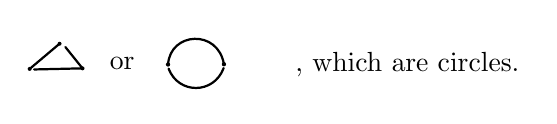
\begin{tikzpicture}[x=1em,y=1em,line cap=round,line join=round]
\draw[thick] (0,0) -- (1.08,.91);
\draw[thick] (1.29,.79) -- (1.91,.02) -- (.16,-.02);
\fill (0,0) circle (.072) (1.08,.91) circle (.072) (1.91,.02) circle (.072);
\node at (3.34,.18) {\handwritten{or}};
\draw[thick] (5,.16) .. controls (5.08,1.34) and (6.80,1.45) .. (7.02,.17);
\draw[thick] (5.02,.01) .. controls (5.37,-.92) and (6.65,-.93) .. (7.01,.03);
\fill (5,.16) circle (.078) (7.02,.17) circle (.078);
\node[anchor=west] at (9.25,.15) {\handwritten{, which are circles.}};
\end{tikzpicture}}
This \deleted{restriction}\inserted{formulation} however has the unconvenience of not being directly expressed in combinatorial terms. The following formulation, which has the advantage of being of combinatorial nature, is presumably equivalent to the former, and gives \deleted{\unsure{enough}} (I expect) \deleted{enough} a large enough notion of ``standartness'' to yield \deleted{\unsure{f}}\unsure{fpr|for} the corresponding notion of $\infty$-category \unsure{enough structure for whatever one will ever need.} \unsure{In any case, it is}
% archive sheet number: 104
